\chapter{Background}
\label{ch:background}

    \section{Computing Continuum}
    \label{sec:computing-continuum-background}

        Placeholder

    \section{Scheduling and Adaptation}
    \label{sec:scheduling-and-adaptation-background}

    \section{Prediction of Load}
    \label{sec:prediction-of-load-background}

    \section{Recurrent Neural Network}
    \label{sec:rnn-background}

        Recurrent neural networks (RNN) were designed to improve upon the shortcomings of traditional neural networks when dealing with sequential data.
        A traditional feed-forward neural network is unidirectional, meaning that they have a single direction and hence cannot persist information over a time step $t$.
        Looping structures are added to a feed-forward neural network that enable the persistance of information about time-series or sequential data. 
        This is the reason RNN's are known as "recurrent" neural networks.
        \cite{datacloudToolbox}

        \begin{figure}[h!]
            \centering
            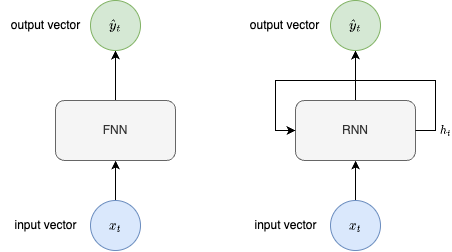
\includegraphics[scale=0.5]{figures/FNN_vs_RNN.drawio.png}
            \caption{Feed-Forward Neural Network vs. RNN}
            \label{fig:fnn-vs-rnn}
        \end{figure}

    \section{Long-Short Term Memory}
    \label{sec:lstm-background}

        \emph{Long-Short Term Memory (LSTM)} are a type of \ref{sec:rnn-background} but improve upon the shortcomings of regular RNN models.
        LSTMs are best suited for learning long term dependencies in sequential or time-series data.

        The introduction of \emph{self-looping} to produce paths is the main architectural improvement for LSTMs over RNNs. This additional component diminishes the problem of the vanishing gradients problem and enables gradients to flow for a long duration.